\chapter{Fenwick Tree}\label{chp:fenwick_tree}

For \verb|range_update| and \verb|point_update| both in $log(n)$ time, we use fenwick tree.
Fenwick tree has very low code footprint. \footnote{but you must understand the tree strucutre and uppdate sequence to understand how it works.}
\footnote{
\href{https://cs.stackexchange.com/questions/10538/bit-what-is-the-intuition-behind-a-binary-indexed-tree-and-how-was-it-thought-a}{link:Intution Behind Fenwick Tree}}
\footnote{fenwick tree is not suitable for range update}

\intution{Intution: Just like carr[] gives us rangeQuery in O(1), but point update is still O(n). What if we store the array element itself in a balanced binary tree, where each node contains the sum of all its left child nodes.}
With this defination, \verb|q[0,idx]| can be done in log(n) time, and so does point update in log(n). (think it like in both the operations we traversal from leaf node to root)
\newpage
% \begin{fullwidth}

%     \begin{figure}
%         \begin{minipage}[c]{0.5\fullwidthlen}
%             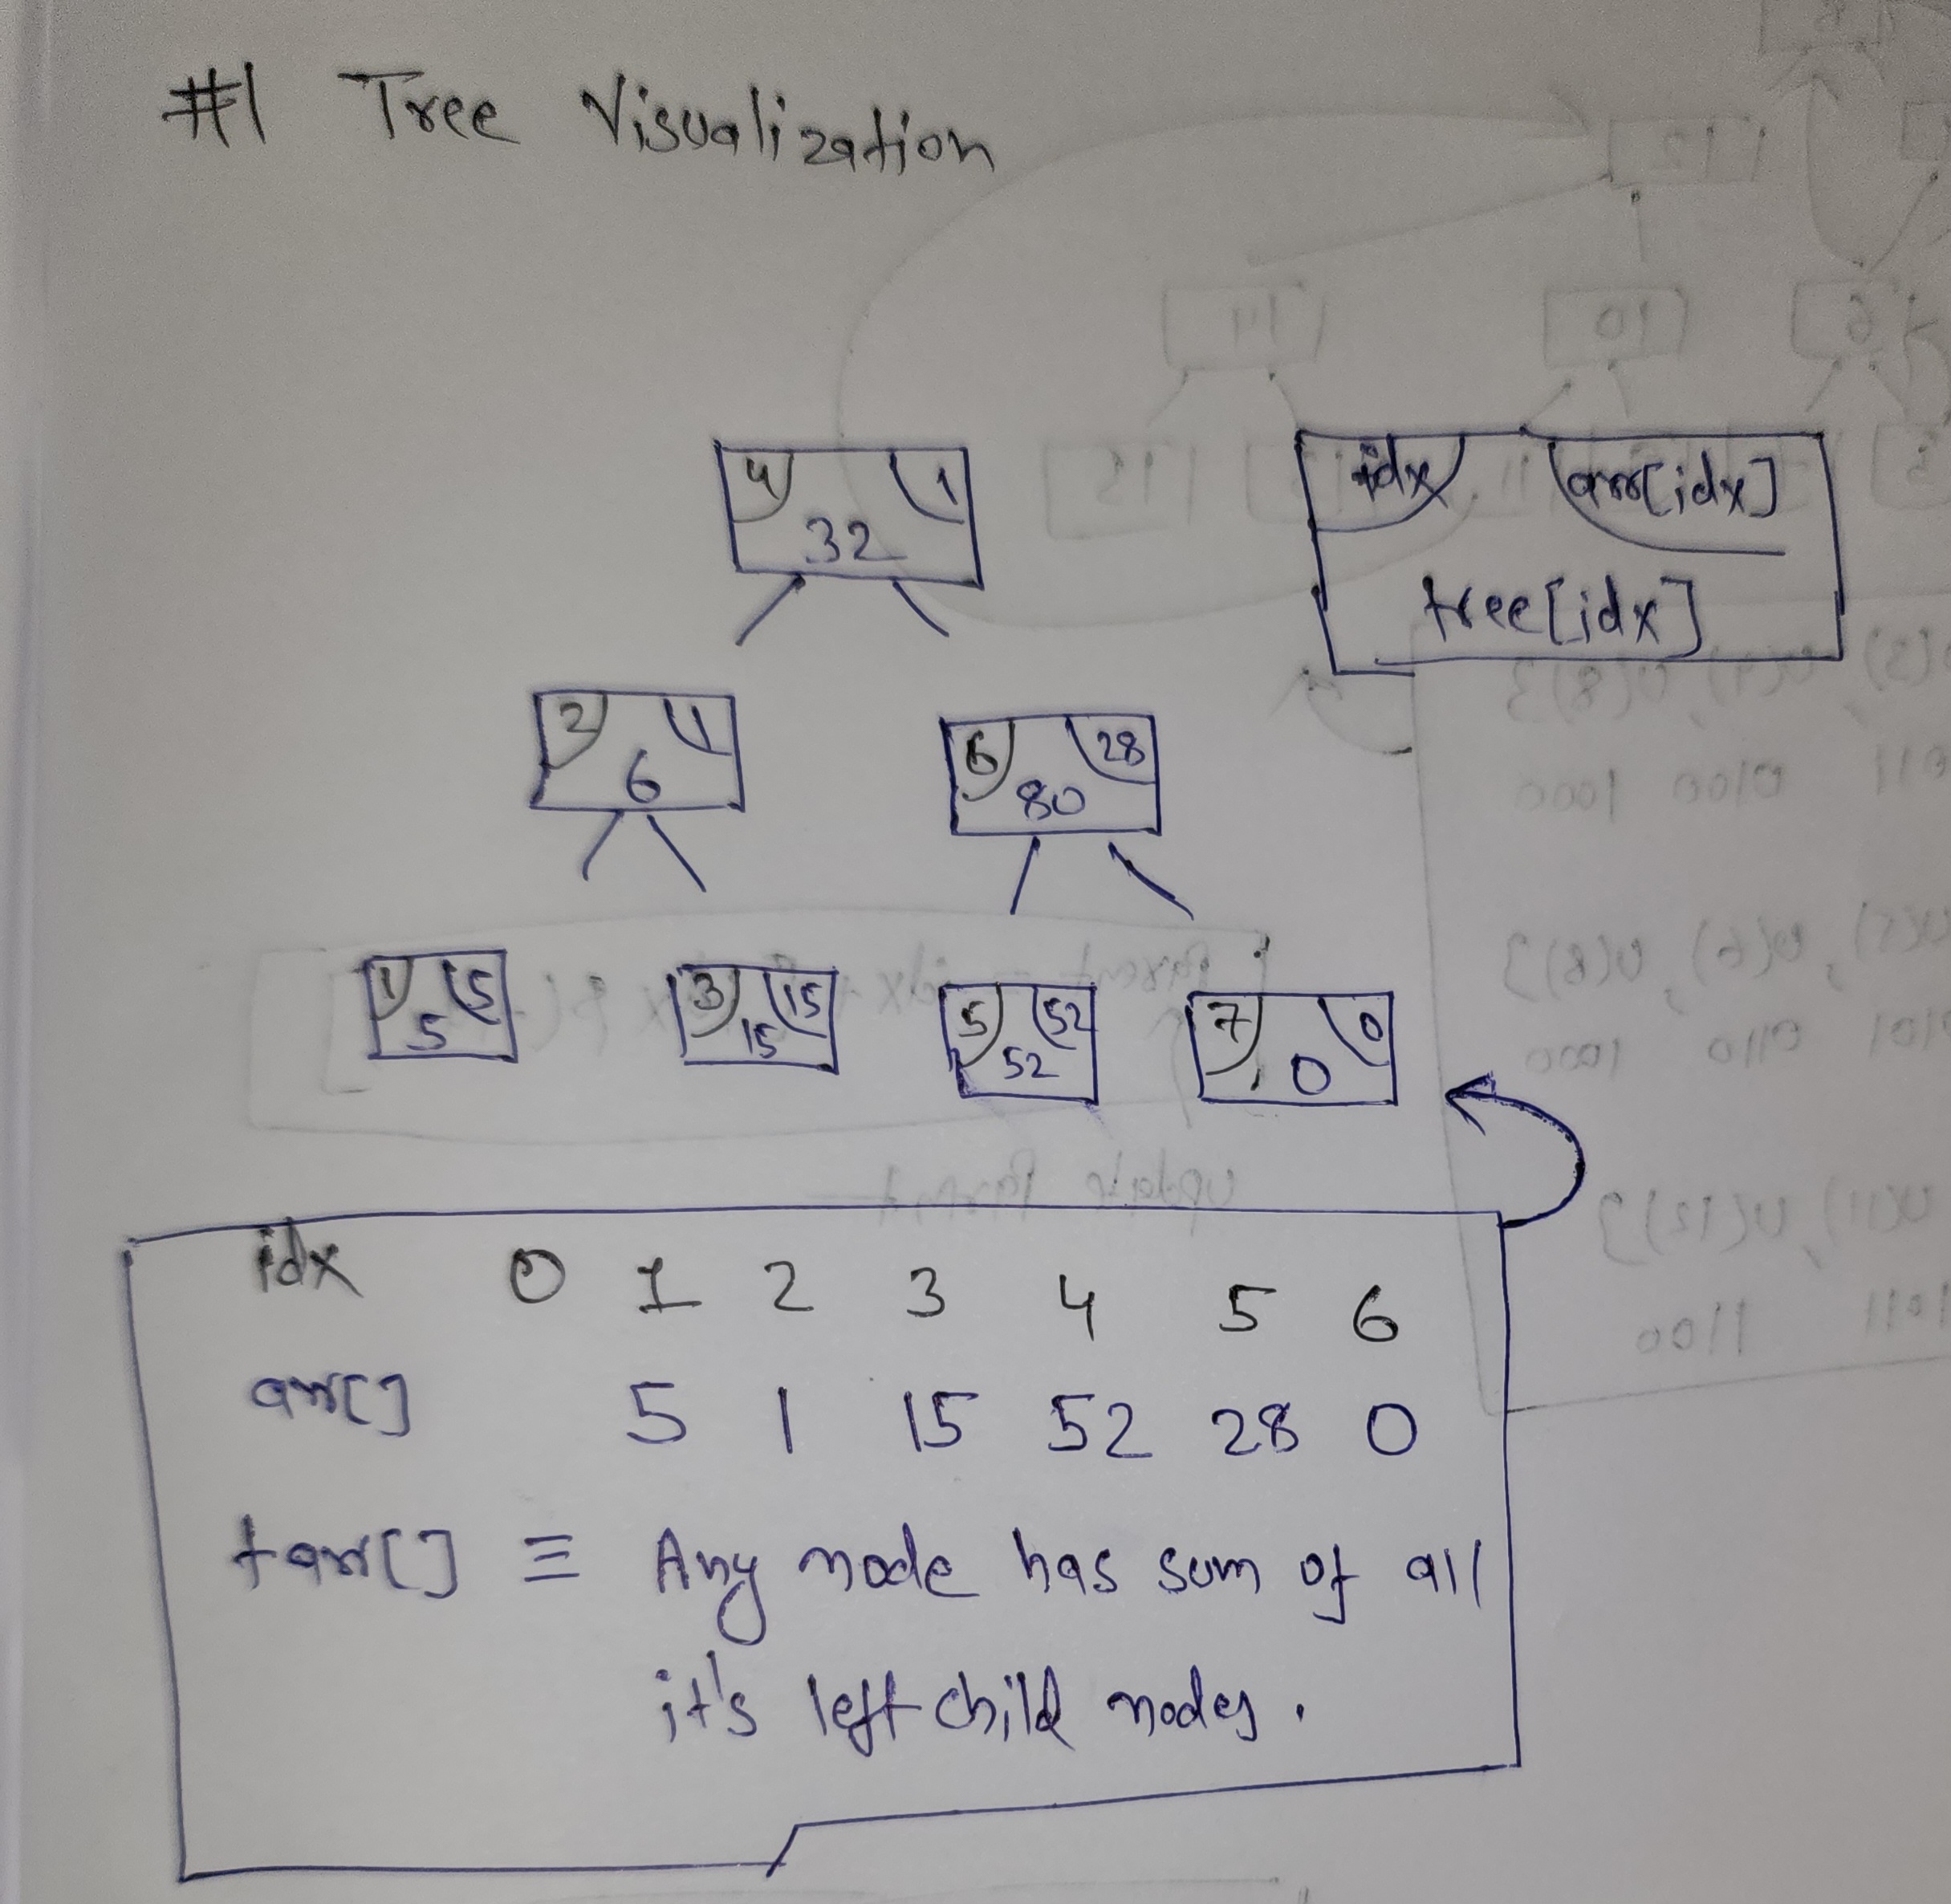
\includegraphics[width=.3\textwidth]{resources/dsa-fenwick-tree-visualization.jpg}
%         \end{minipage}
%         \begin{minipage}[c]{0.3\fullwidthlen}
%           \caption{some caption}
%         \end{minipage}

%       \end{figure}

      
% \end{fullwidth}


    % \begin{figure}
    %     \begin{fullwidth}
    %     \begin{minipage}[c]{0.4\fullwidthlen}
    %         \includegraphics[width=\textwidth]{example-image}
    %     \end{minipage}\hspace{5mm}
    %     \begin{minipage}[c]{0.6\fullwidthlen}
    %            \lipsum[2]
    %            % Hello
    %     \end{minipage}
    % \end{fullwidth}
    % \end{figure}

\codecaption{Fenwick Tree Visualization/Debug}
\begin{lfigure}{resources/dsa-fenwick-tree-visualization.jpg}{0.6}{0.38}
    Any node in the tree has sum of all node in its leftsubtree.
    \vspace{1cm}

    \verb|query_parent = idx + [idx & (-idx)]|

    \verb|update_parent = idx - [idx & (-idx)]|

    \vspace{2cm}
    Class Skeleton
    \begin{code3}

    vector<treeNode> tree;
    lli treeSize;

    public:
    FT(vector<lli>& arr)
    {
        treeSize = arr.size()+1;
        tree = 
        vector<treeNode>(treeSize)
    }
    \end{code3}

\end{lfigure}

\codecaption{Point Update with Fenwick Tree}
\begin{lfigure}{resources/dsa-fenwick-point-update.jpg}{0.5}{0.5}

    \begin{code3}
    void update(lli idx, lli val)
    {
        tree[idx].val += val;

        while(idx <= treeSize)
        {
            tree[idx].lsum += val;
            idx = update_parent_idx(idx);
        }
    }

  
    inline lli update_parent_idx(lli idx)
    {
        return  idx + (idx & (-idx));
    }
    \end{code3}

\end{lfigure}

\codecaption{Range Query}
\begin{lfigure}{resources/dsa-fenwick-range-query.jpg}{0.5}{0.5}
    \begin{code3}
    lli query(lli idx)
    {
        lli sum = 0;
        lli p = 0;
        while(idx>0)
        {
            sum += tree[idx].lsum;
            idx = idx - (idx & (-idx));        
        } 
        return sum;
    }
    
    lli range_query(lli left,lli right)
    {
        return query(right) - query(left-1);
    }
    \end{code3}
\end{lfigure}